\documentclass[a4paper,12pt]{report}

\usepackage{a4wide}
\usepackage[dutch]{babel}
\usepackage[utf8]{inputenc}
\usepackage[dvipsnames]{xcolor}
\usepackage{graphicx}
\graphicspath{ {images/} }
\usepackage[small,bf,hang]{caption}
\usepackage{amsmath}
\usepackage{siunitx}
\usepackage{cite}
\usepackage{hyperref}
\usepackage{tocbibind}
\usepackage{pgfgantt}
\usepackage[gen]{eurosym}

\begin{document}

\title{
	{
\includegraphics{UGent_FEA_Logo.png}}\\
	{Voorraadbeheer in magazijnen}\\
	{\large Universiteit Gent}\\
	{
\includegraphics{UGent_Logo.png}}
}	
\author{Xavier Claerhoudt\\
\texttt{Xavier.Claerhoudt@UGent.be}
\and Bram De Smet\\
\texttt{Bram.DeSmet@UGent.be}
\and Robbe De Vilder\\
\texttt{Robbe.DeVilder@UGent.be}
\and Garben Tanghe\\
\texttt{Garben.Tanghe@UGent.be}
\and \textit{3\textsuperscript{de} Bachelor Computerwetenschappen}}
\date{21 mei 2018}
\maketitle

\pagenumbering{roman}

\tableofcontents
\listoffigures
\listoftables

\begin{abstract}
Het doel van dit project is om commercieel beschikbare drones te voorzien van een functionele on-board controller en gebruik te maken van een controlebord dat instaat voor de drone-aansturing en -lokalisatie.\\
Daarnaast is de controller verantwoordelijk voor communicatie met een centraal controlepunt.\\
Tegen het eind van het project moet de drone in staat zijn om autonoom en probleemloos een vanuit het controlepunt verzonden route af te leggen.
\end{abstract}

\pagenumbering{arabic}
\chapter{Analyse van de probleemstelling}
Voorraadbeheer in een magazijn gebeurt traditioneel door werknemers die op een vorklift handmatig barcodes inscannen. Zoals u kan aanvoelen is dat een zeer langzame, dure en gevaarlijke aanpak. Een kosteneffectievere oplossing is het gebruikmaken van automatisch aangestuurde drones die met een camera de barcodes kunnen inscannen.\\

Het doel van dit vakoverschrijdend project is om een basis te leggen voor dit systeem. In eerste instantie is het doel om een drone een vooraf bepaalde route autonoom te laten vliegen in een magazijn.\\
Later kunnen dan uitbreidingen op dit project gemaakt worden. Voorbeelden van mogelijke uitbreidingen zijn: een wifi-mesh van meerdere drones en een functionele RFID scanner die de gescande codes naar het centrale controlepunt verstuurd.
\chapter{Planning}

\section{Initi\"ele planning} \label{sec:initiele_planning}
De initi\"ele planning is terug te vinden op figuur \ref{fig:initiele_planning}.
\begin{figure}[p]
\centering
\begin{ganttchart}[vgrid, y unit chart=0.75cm, bar/.append style={fill=White, rounded corners=2pt}, milestone/.append style={fill=White}]{1}{13}
	\gantttitlelist{1,...,13}{1}\\

	\ganttgroup{Hardware}{1}{5}\\
	\ganttbar{Uitzoeken en bestellen}{1}{2}\\
	\ganttbar[bar/.append style={fill=JungleGreen}]{Raspberry en DecaWave verbinden}{5}{5}\\
	\ganttbar[bar/.append style={fill=RedOrange}]{Power supply}{5}{5}\\
	\ganttbar[bar/.append style={fill=RedOrange}]{Controller aan drone bevestigen}{5}{5}\\

	\ganttgroup{Software}{3}{12}\\
	\ganttbar[bar/.append style={fill=Yellow}]{UWB}{3}{4}\\
	\ganttbar[bar/.append style={fill=Fuchsia}]{Connectie met server}{5}{6}\\
	\ganttbar[bar/.append style={fill=Fuchsia}]{Aansturing drone}{4}{9}\\
	\ganttbar{Full-mesh}{10}{12}\\

	\ganttgroup{Presentaties en verslag}{1}{13}\\
	\ganttmilestone[milestone/.append style={fill=JungleGreen}]{Presentatie 1}{4}\\
	\ganttlinkedmilestone[milestone/.append style={fill=RedOrange}]{Presentatie 2}{8}\\
	\ganttlinkedmilestone{Verslag}{12}\\
	\ganttlinkedmilestone{Eindpresentatie}{13}
\end{ganttchart}
\caption[Gantt chart van de initi\"ele planning.]{Gantt chart van de initi\"ele planning.}
\label{fig:initiele_planning}
\end{figure}

\section{Taakverdeling} \label{sec:taakverdeling}
Wie doet wat? Dit kun je terug vinden in tabel \ref{tab:taakverdeling}.
\begin{table}[p]
\centering
\begin{tabular}{ |c|c|c| } \hline
Wat? & Wie? & Kleur \\ [.5ex] \hline\hline
Uitzoeken en bestellen & Iedereen & WIT \\ \hline
Power supply & Garben & ROODORANJE \\ \hline
UWB & Bram & GEEL \\ \hline
Visualisatie & Xavier & SEPIA \\ \hline
Connectie met server & Iedereen & WIT \\ \hline
Aansturing drone & Robbe & FUCHSIA \\ \hline
Presentatie 1 & Bram en Garben & JUNGLEGROEN \\ \hline
Presentatie 2 & Robbe en Xavier & BLAUW \\ \hline
Verslag & Iedereen & WIT \\ \hline
Eindpresentatie & Iedereen & WIT \\ \hline
\end{tabular}
\caption[Taakverdeling]{Taakverdeling.}
\label{tab:taakverdeling}
\end{table}

\section{Finale planning} \label{sec:finale_planning}
De finale planning is terug te vinden op figuur \ref{fig:finale_planning}.
\begin{figure}[p]
\centering
\begin{ganttchart}[vgrid, y unit chart=0.75cm, bar/.append style={fill=White, rounded corners=2pt}, milestone/.append style={fill=White}]{1}{13}
	\gantttitlelist{1,...,13}{1}\\
	
	\ganttgroup{Hardware}{1}{5}\\
	\ganttbar{Uitzoeken en bestellen}{1}{2}\\
	\ganttbar[bar/.append style={fill=JungleGreen}]{Raspberry en DecaWave verbinden}{5}{5}\\
	\ganttbar[bar/.append style={fill=RedOrange}]{Power supply}{5}{5}\\
	\ganttbar[bar/.append style={fill=RedOrange}]{Controller aan drone bevestigen}{5}{5}\\
	
	\ganttgroup{Software}{3}{12}\\
	\ganttbar[bar/.append style={fill=Yellow}]{UWB}{3}{4}\\
	\ganttbar[bar/.append style={fill=Fuchsia}]{Connectie met server}{5}{6}\\
	\ganttbar[bar/.append style={fill=Fuchsia}]{Aansturing drone}{4}{9}\\
	\ganttbar{Full-mesh}{10}{12}\\
	
	\ganttgroup{Presentaties en verslag}{1}{13}\\
	\ganttmilestone[milestone/.append style={fill=JungleGreen}]{Presentatie 1}{4}\\
	\ganttlinkedmilestone[milestone/.append style={fill=RedOrange}]{Presentatie 2}{8}\\

	\ganttlinkedmilestone{Verslag}{12}\\
	\ganttlinkedmilestone{Eindpresentatie}{13}
\end{ganttchart}
\caption[Gantt chart van de finale planning.]{Gantt chart van de finale planning.}
\label{fig:finale_planning}
\end{figure}\\

De grootste verschillen tussen de initi\"ele planning en de finale planning zijn ...\\

De motivatie van de belangrijkste wijzigingen zijn ...
\chapter{Hardware}
In wat volgt, worden alle componenten uitvoerig besproken en wordt een verantwoording gegeven van de ontwerpskeuzes.

\section{Drone} \label{sec:drone}
De eerste beslissing omtrent hardware was het uitzoeken van de drone. Hier werd geopteerd voor de Parrot AR.Drone 2.0 Elite Edition met jungle camo. De belangrijkste argumenten voor deze keuze zijn de kostprijs en de grootte.\\

Vaak kosten drones die een lading van zo'n \SI{100}{\g} kunnen dragen minstens \SI{250}{\euro{}}. Dit type is echter al even niet meer in productie, waardoor de prijs enorm gezakt is. Een goedkopere drone, die niet onder de minidrones geplaatst wordt, kon niet gevonden worden.\\

Ook voor het software gedeelte is deze drone een goede keuze. Parrot stelt een SDK openbaar ter beschikking en er bestaan reeds libraries, waarvan er in dit project ook gebruik gemaakt wordt.\\
De camera op de drone zou kunnen dienen om barcodes in te scannen, maar dat onderdeel werd niet onder de doelstellingen van dit project gedefini\"eerd.\\
Tot slot bezit de drone ook nog een ultrasone sensor om de hoogte t.o.v. de vloer te meten en een camera om stabiel te blijven zweven op dezelfde positie.

\section{Indoor lokalisatie}  \label{sec:uwb}
In theorie is het mogelijk om, als een drone op een gekende locatie (met een gekende ori\"entatie) vertrekt, deze zonder enige input informatie of correcties een reeks vluchtbewegingen door te geven zodat een voorgeprogrammeerde route gevolgd wordt. In de praktijk wordt dit echter bemoeilijkt door ongekende externe factoren, denk bijvoorbeeld maar aan een ongekend obstakel dat plots het pad van de drone kruist, of een ventilatieschacht die de drone uit positie blaast. Ook het opstijgen gebeurt niet vlekkeloos, waardoor hij met een foutieve ori\"entatie aan zijn tocht zou beginnen. Daarom is het nodig dat het toestel z'n specifieke locatie in de ruimte op elk moment gekend is. \\

Als de drone tussen 2 rekken met een doorgang van \SI{1}{\m} moet kunnen vliegen, dan moet de nauwkeurigheid van lokalisatie in de grootte orde van \SI{0.10}{\m} liggen. Veelgebruikte lokalisatie-technologie\"en zoals gps, wifi en bluetooth zijn te onnauwkeurig voor deze toepassing. Ultra Wide Band komt deze noden tegemoet. Dit is een vrij recente techniek met een nauwkeurigheid in de grootteorde van \SI{0.10}{\m}, wat volstaat om de drone indoor te kunnen lokaliseren.\\

Voor de locatiebepaling werd beroep gedaan op de Pozyx-hardware\footnote{\url{https://www.pozyx.io}}, ontwikkeld door een spin-off van de Ugent, meer bepaald op de anker nodes (die op gekende locaties in de ruimte worden opgehangen) en op een mobiele tag (die als onderdeel van de controller op de drone wordt bevestigd). 
Over de mobiele tag is meer te vinden in sectie \ref{sec:pozyx_tag}.

\section{On-board Controller} \label{sec:onboard_controller}

De locatiebepaling gebeurt via een controller die we op de drone monteren, deze bestaat uit een Pozyx tag, een Raspberry Pi Zero W en een batterij.

\subsection{Pozyx tag}  \label{sec:pozyx_tag}
De mobiele tag kan om de beurt de verschillende ankers aanspreken, en opvragen hoe ver hij van hen verwijderd is. Wanneer er enkele van deze afstanden gekend zijn, kan hij zijn locatie bepalen ten opzichte van de ankers.\\

Er werden twee verschillende opties vergelijken (zie tabel \ref{tab:decavspozyx}) als mogelijke UWB component: DecaWave DWM1001 en Pozyx. De DecaWave is een goedkope, lichte en compacte module. Echter zou het implementeren van de lokalisatie geen makkelijk programmeertaak zijn, mede doordat de communicatie met de chip niet evident is. Ook waren deze module niet direct beschikbaar. Hierdoor is er gekozen voor de duurdere, zwaardere en grotere pozyx tag. Deze waren direct beschikbaar, en ook de begeleiders hadden hier reeds ervaring mee. Voor de gebruikte drone is het minieme gewichtsverschil niet echt een probleem. Men moet echter wel in het achterhoofd houden dat meer massa de stabiliteit en vliegminuten in negatieve zin be\"invloedt.\\

\begin{table}[p]
\centering
\begin{tabular}{ | l | c | c | } \hline
& DecaWave DWM1001 & Pozyx \\
\hline 
\hline
Prijs (\euro{}) & 20 & 135 \\ 
\hline
Massa (g) & 4 & 12 \\ 
\hline
Afmetingen ($mm \times mm$) & $19.1 \times 26.2$ & $60 \times 53$ \\ 
\hline
\end{tabular}
\caption[Vergelijking DecaWave DWM1001 Module en Pozyx tag]{Vergelijking DecaWave DWM1001 Module en Pozyx tag}
\label{tab:decavspozyx}
\end{table}

\subsection{Raspberry Pi Zero W} \label{sec:raspberry_pi}

Het aansturen van de Pozyx tag gebeurt met een Raspberry Pi Zero W. 

\subsection{LiPo Batterij en Power Supply} \label{sec:lipo}
De Lithium-ion Polymeer Batterij (LiPo) moet de controller gedurende ongeveer een kwartier van stroom kunnen voorzien, aangezien de drone ook ongeveer \SI{15}{\min} lang in de lucht kan blijven.\\
De controller heeft gedurende een kwartier ongeveer \SI{350}{\mA} nodig. Om pieken op te kunnen vangen werd gekozen voor een batterij van \SI{500}{\mA\hour}. Deze kan gedurende een kwartier zo'n \SI{2000}{\mA} leveren aan de controller.\\

Omdat de Rasberry Pi Zero W op \SI{5}{\V} opereert i.p.v. op de \SI{3.7}{\V} van de LiPo batterij, wordt er nog een LiPo SHIM tussen geplaatst. Deze zal niet enkel het voltage omvormen, maar bezit ook een indicator dat inschakelt wanneer de batterij bijna leeg is.

\section{Off-board Controller} \label{sec:offboard_controller}
Om de drone effectief aan te sturen maken we gebruik van een Raspberry Pi 3 B. Deze heeft de mogelijkheid om met 2 netwerken tegelijk te verbinden. De Ethernet interface wordt gebruikt om verbinding te maken met het internet (en de MQTT server), terwijl de wifi interface gebruikt wordt om met het netwerk van de drone te verbinden.

\section{Setup} \label{sec:setup_hardware}
Op figuur \ref{fig:setup_hardware} vindt u de hardware setup.
\begin{figure}[p]
	\centering
	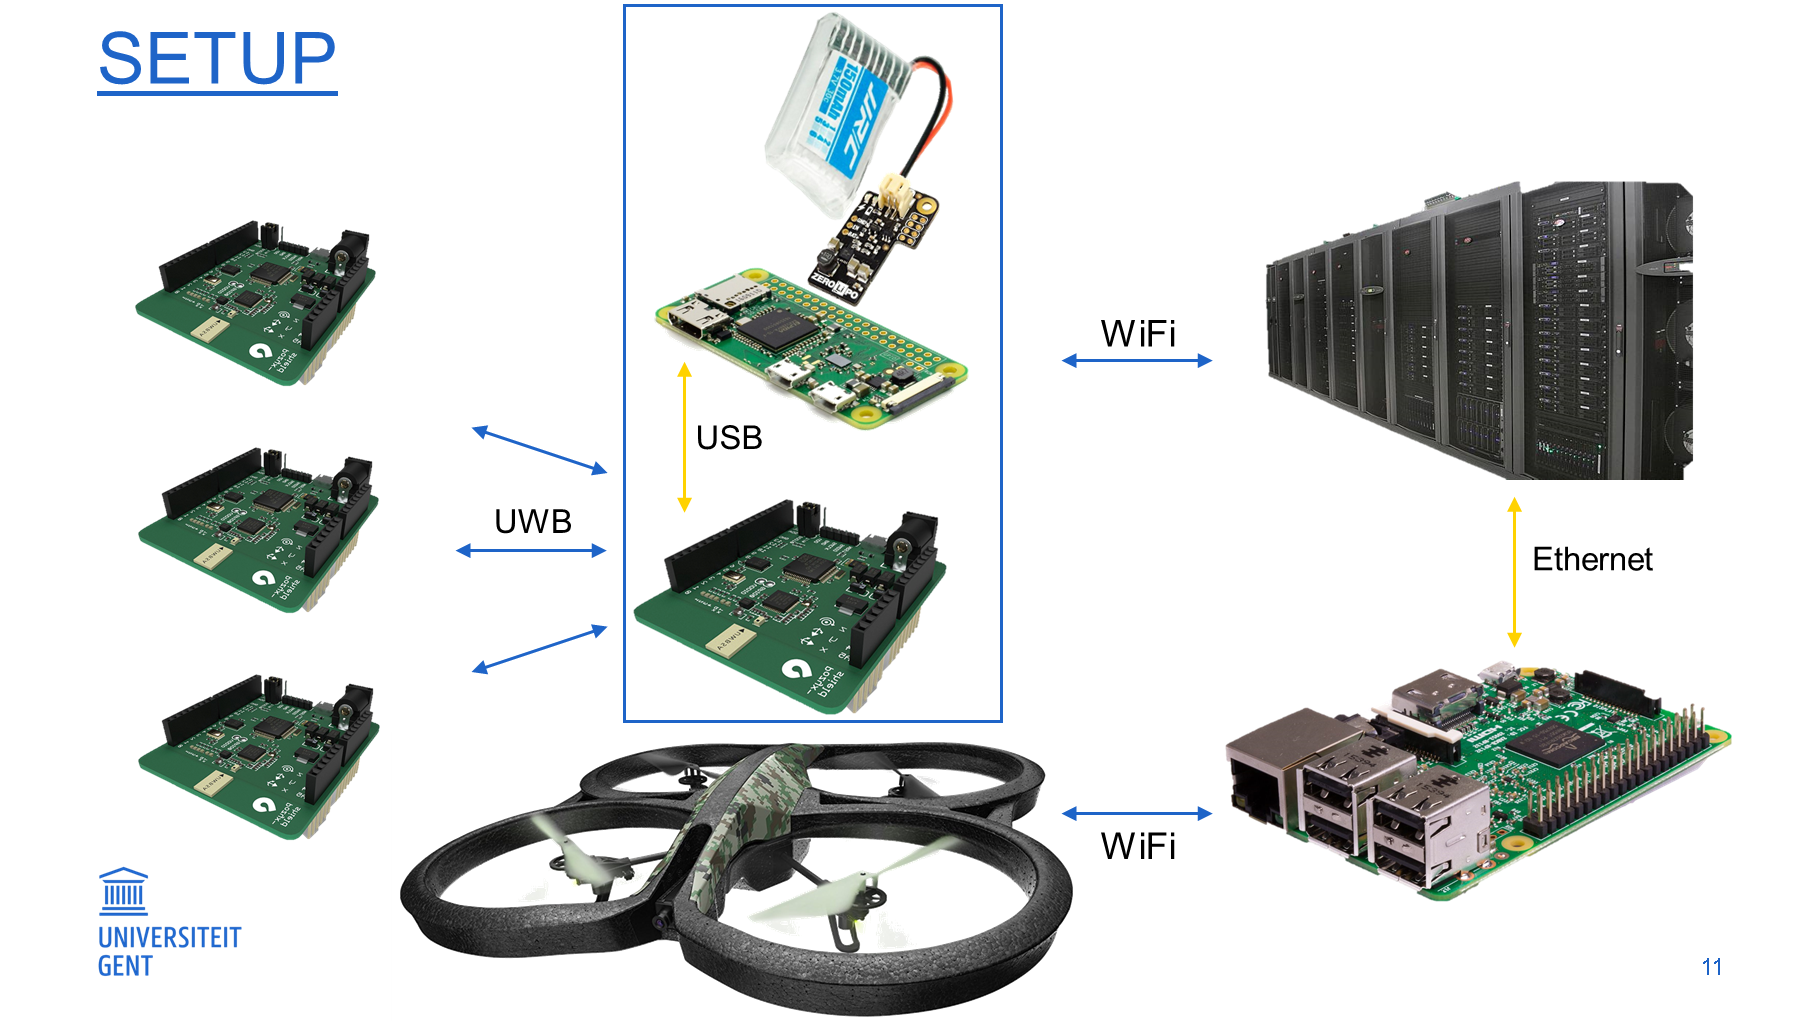
\includegraphics[width=\textwidth]{Setup_Hardware}
	\caption[Hardware setup]{Hardware setup.}
	\label{fig:setup_hardware}
\end{figure}
\chapter{Software}
In wat volgt, wordt het ontwerpproces van de software uitvoerig besproken en wordt een verantwoording gegeven van de ontwerpskeuzes.

\section{Verbinding tussen de UWB location anchors en tag} \label{sec:uwb_tag}
Ultra Wide Band (UWB) \cite{uwb2016}.\\

Een belangrijk aspect naast nauwkeurigheid, is de snelheid.
We zullen dus ook een algoritme moeten schrijven die bepaalt op welke ankers hij zich basseert.
Het zou een beetje over-kill zijn als hij alle ankers in het volledige magazijn aanspreekt voor zijn locatie.
Een mogelijke manier zou zijn dat we op voorhand bepalen dat hij gebruik maakt van het anker waar hij zich het dichtst bij bevindt en 4 ankers die zich in de buurt bevinden.\\

Nog een element die we in rekening moeten brengen is dat de server mogelijks enkel 2D ondersteunt, wat dus niet voldoet voor een drone die op verschillende hoogtes kan vliegen.
Gelukkig zit er in de drone een ultrasone sensor en een barometer ingebouwd die zijn hoogte kan bepalen.

\section{Verbinding tussen de Raspberry Pi Zero W en de server} \label{sec:raspberry_server}
Wanneer de controller afstanden ontvangt tot gekende ankers, moeten deze nog verwerkt worden tot de correcte locatie binnen de ruimte.
Hiervoor kunnen we gebruik maken van een Mosquitto server die deze complexe berekeningen op zich neemt.
Communicatie met de Mosquitto server werkt via het MQTT protocol.\\

\section{Verbinding tussen de server en de Raspberry Pi 3 B} \label{sec:server_raspberry}
De off-board controller zal via dat zelfde MQTT protocol posities van de drone en van de waypoints van de server verkrijgen.
Op deze plaats wordt dan een algoritme uitgevoerd dat de aansturingsinstructies voor de drone zal bepalen en uiteindelijk ook versturen.\\

Hier hebben we 2 algoritmes voor geschreven:\\
In het eerste algoritme zal de drone enkel draaien rond de z-as en voorwaarts bewegen als hij in de juiste richting kijkt.
Natuurlijk kan de drone nog steeds op en neer bewegen langs de z-as, onafhankelijk van de bewegingen in het xy-vlak.
Eerst draaien en dan pas zich naar voor verplaatsen is een vrij trage manier om in een kamer te bewegen.
Deze bewegingen kunnen niet tegelijk gebeuren of de drone wijkt al snel af van z'n oorsponkelijk pad.\\
In een tweede algoritme zal de drone nooit draaien.
Hij zal enkel naar voor, achter, links rechts, op een neer bewegen.
Uiteraard worden ook kleine correcties aangebracht om de voorkant van de drone steeds in de juiste richting te doen wijzen.
Deze methode is een hoop sneller, omdat er meer richtingen zijn waarin de drone zich kan voortbewegen.\\

Bij beide algoritmes probeert de drone om een reeks targets \'e\'en voor \'e\'en te bezoeken, eerder dan een bepaald traject binnen een bepaalde tijd af te leggen.
Pas zodra een target bezocht is, gaat de drone naar de volgende plek.
Er worden dus geen waypoints over geslaan als de drone achter raakt op schema.\\
In de praktijk kunnen deze waypoints overeenkomen met dozen die gescand moeten worden.\\
Dit betekent ook dat collision detection tussen mogelijks kruisende drones ook live dient te gebeuren, om te voorkomen dat drones die voor of achter of schema zijn tegen elkaar vliegen.

\section{Verbinding tussen de Raspberry Pi 3 B en de drone} \label{sec:raspberry_drone}
De drone zet een eigen wifi-netwerk met ESSID adrone2\_XXXXXX  op en geeft zichzelf vaak het IP-adres 192.168.1.1.
Als de Raspberry Pi 3 B verbindt met het netwerk van de drone, krijgt het een IP-adres tussen 192.168.1.2 en 192.168.1.5 (met de grenzen inbegrepen) toegekend.
Indien de drone een ander IP-adres aan zichzelf toegekend heeft, zullen de gebruikers één van de 4 volgende adressen toegekend krijgen.\\
Het besturen van de drone gebeurd door het versturen van \textit{AT commands} op UDP poort 5556.
De maximale frequentie waarmee de commando's kunnen doorgestuurd worden ligt rond de \SI{30}{\Hz}, om de drone snel te kunnen laten reageren, en een goede gebruikerservaring te garanderen.\\

Informatie over de drone (zoals status, positie, snelheid, snelheid van de rotoren, ...) wordt naar de gebruiker gestuurd op UDP poort 5554.
De frequentie waarmee deze \textit{navdata} wordt verstuurd ligt tussen de \SI{15}{\Hz} (in demo mode) en \SI{200}{\Hz} in full (debug) mode.\\
Om belangrijke data, zoals informatie voor de configuratie, te versturen maakt men geen gebruik van UDP, maar van TCP.
Dit gebeurd via de \textit{control port} 5559. \cite{developer_guide2012}\\
De AT commands en navdata worden gestuurd en ontvangen a.d.h.v. een library.

\section{Setup} \label{sec:setup_software}
Op figuur \ref{fig:setup_software} vindt u de hardware setup, aangevuld met protocollen.
\begin{figure}[p]
	\centering
	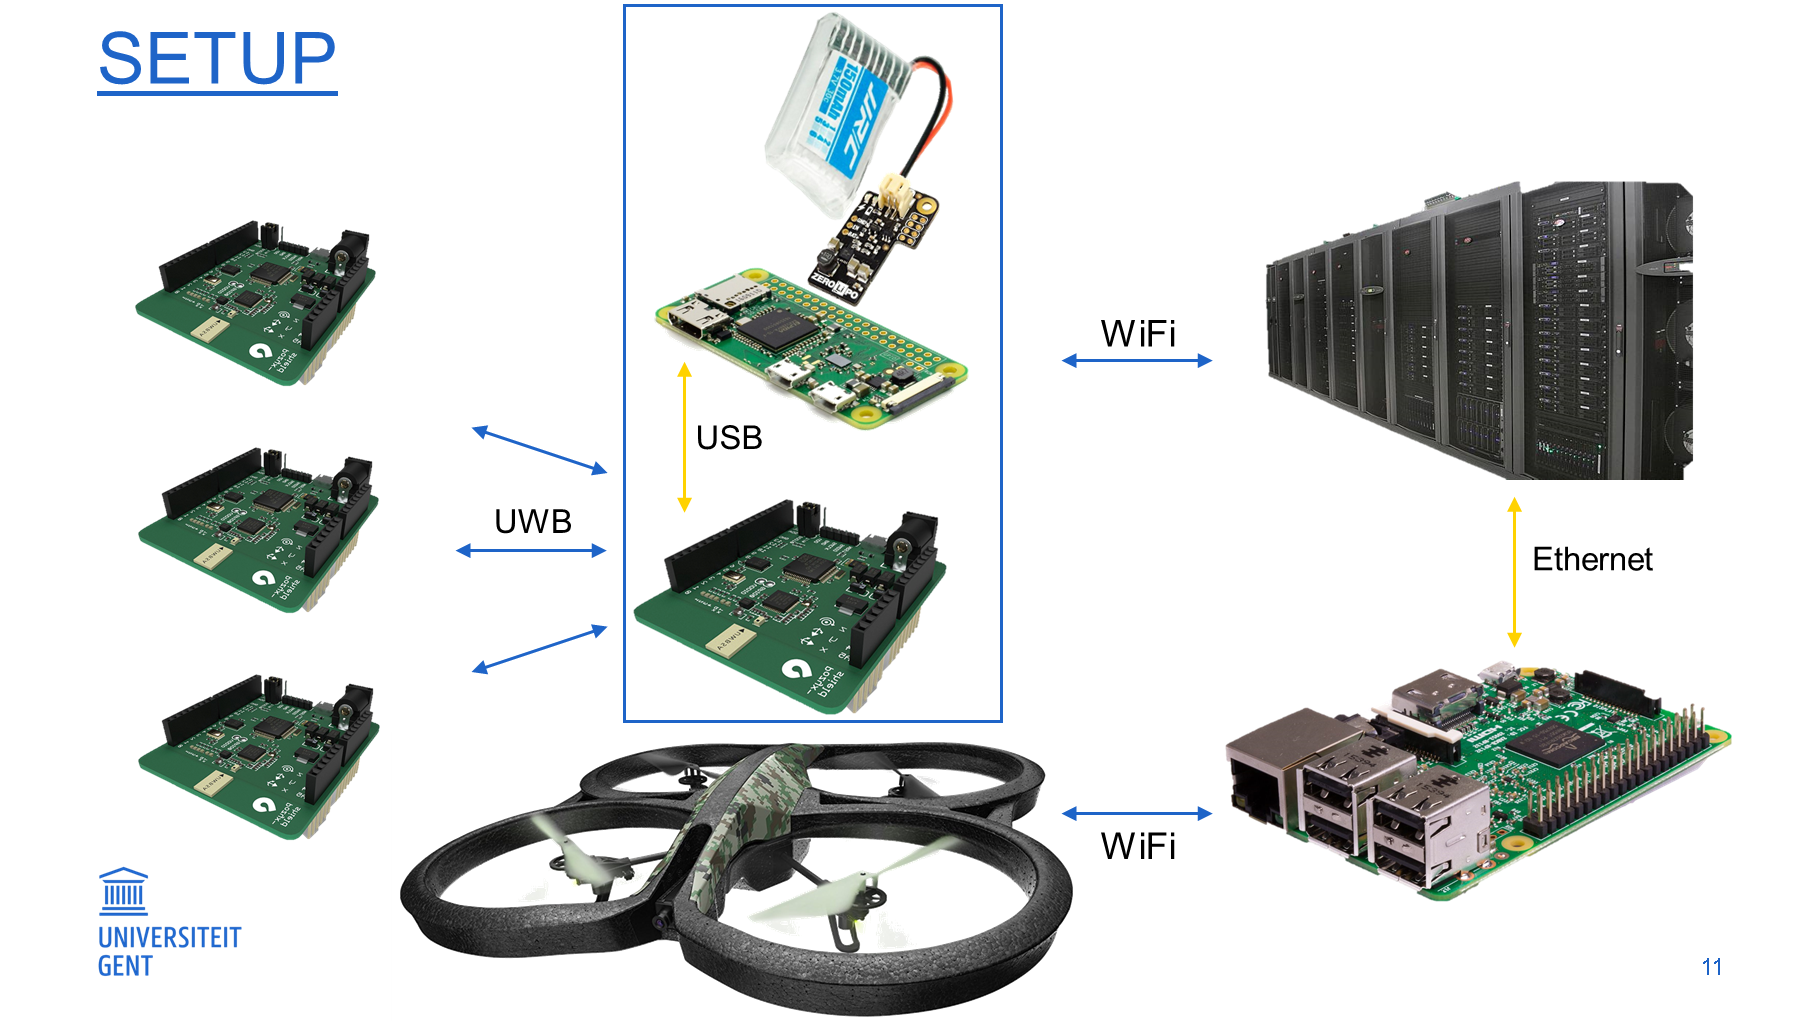
\includegraphics[width=\textwidth]{Setup}
	\caption[Hardware setup, aangevuld met protocollen]{Hardware setup, aangevuld met protocollen.}
	\label{fig:setup_software}
\end{figure}

\section{Visualisatie} \label{sec:visualization}

\chapter{Resultaten}
Het belangrijkste resultaat is natuurlijk de implementatie van het volledige drone systeem. Hierbij vinden er locatie-updates plaats met een frequentie van \SI{27.5}{\Hz} en wordt de drone aangestuurd met een frequentie van \SI{10}{\Hz}.\\

Tijdens de proefopstelling is er gebruik gemaakt van vier pozyx ankers voor de locatiebepaling. Het doel was dat de drone een op voorhand gedefini\"eerd pad vloog, weergegeven met de witte lijnen op figuur \ref{fig:Opstelling}. Op de figuren \ref{fig:SuccesfullFlight1} en  \ref{fig:SuccesfullFlight2} staan de waypoints en de effectief gevlogen paden van twee verschillende testvluchten gevisualiseerd. De waypoints (rode plustekens) komen overeen met de hoekpunten van de rechthoek voorgesteld op figuur \ref{fig:Opstelling}. Rond elk waypoint is een cirkel getekend die de grootte van het waypoint weergeeft, hier $150mm$. Wanneer de drone binnen dit bereik valt, heeft hij het waypoint bereikt. De stippellijnen op komen overeen met de tegels van de ruimte, deze zijn $600mm \times 600mm$. De drone probeert de waypoints de doorlopen in wijzerzin, met het de linkerbovenhoek als startpunt. 

\begin{figure}[p]
	\centering
	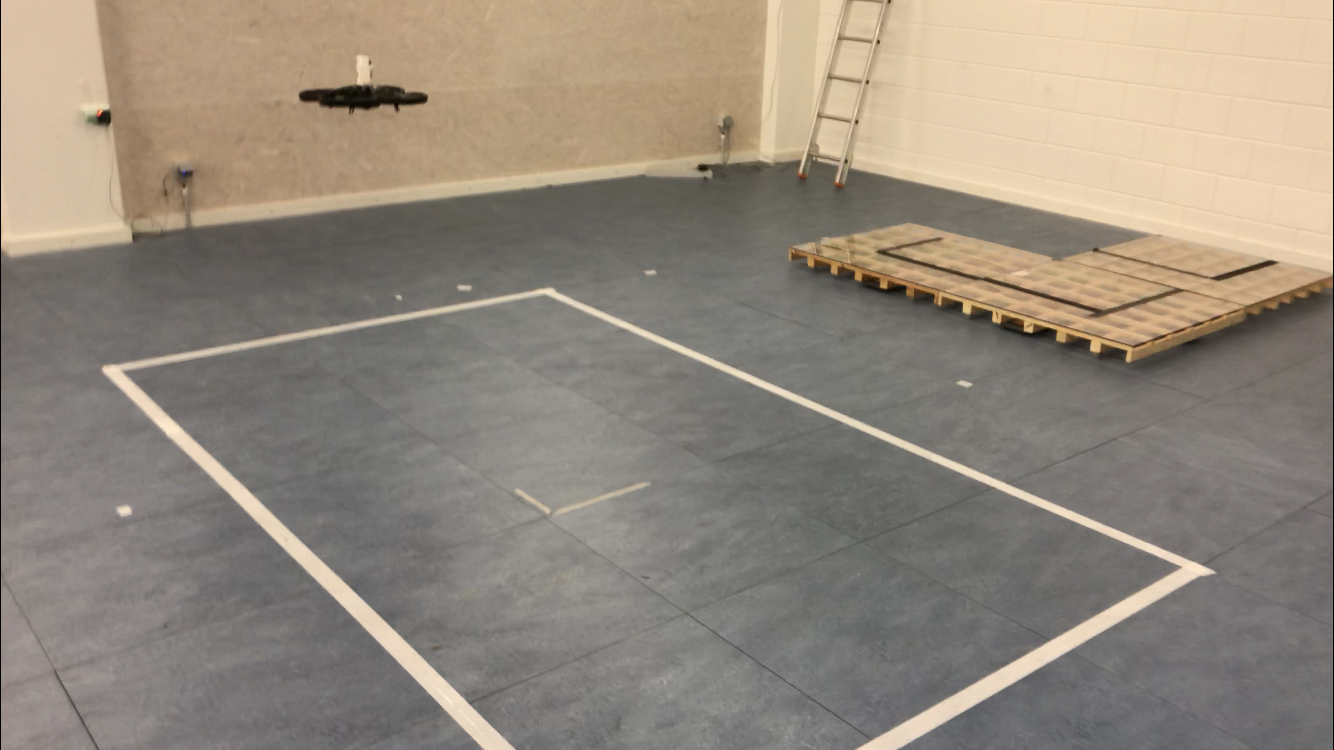
\includegraphics[width=\textwidth]{Opstelling}
	\caption[Opstelling testvluchten]{Testopstelling voor aansturen van de drone.}
	\label{fig:Opstelling}
\end{figure}

\begin{figure}[p]	
	\centering
	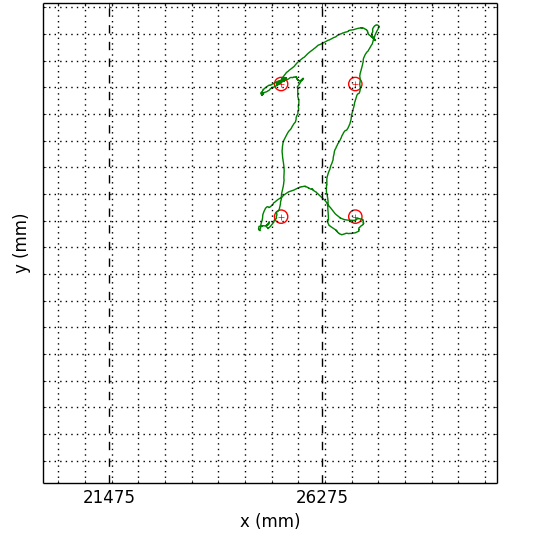
\includegraphics[width=\textwidth]{SuccesfullFlight1}
	\caption[Testvlucht1]{Testvlucht van de drone waarbij hij langs de vier waypoints passeert. }
	\label{fig:SuccesfullFlight1}
\end{figure}
	
\begin{figure}[p]
	\centering
	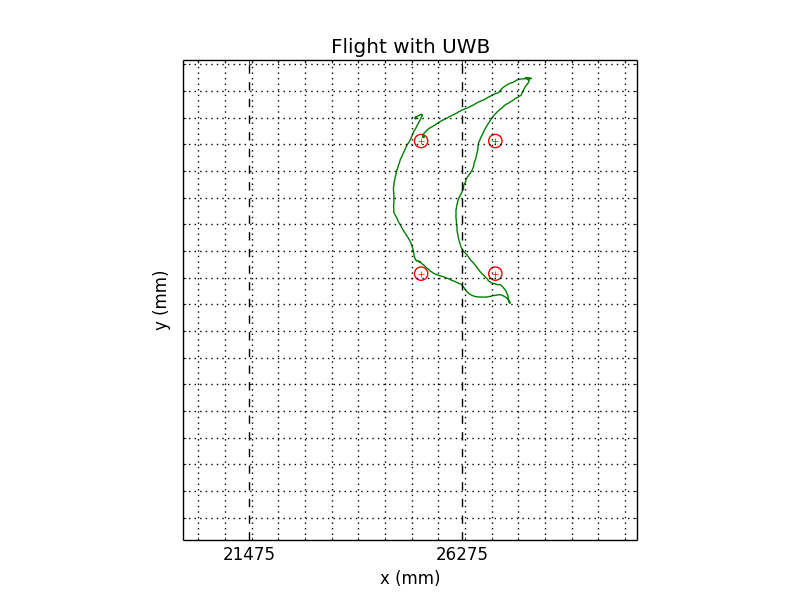
\includegraphics[width=\textwidth]{SuccesfullFlight2}
	\caption[Testvlucht2]{Testvlucht}
	\label{fig:SuccesfullFlight2}
	
\end{figure}

\section{Testen} \label{sec:test}
Indien u dit project zelf wil gebruiken of testen, bezoek dan zeker de git repository\footnote{\url{https://github.ugent.be/gartangh/VOP_Voorraadbeheer}}.

\section{Problemen} \label{sec:problems}
Een openstaand probleem van het project is dat het verbinden van de off-board controller met 2 verschillende netwerken nog niet optimaal verloopt. Vaak wil de applicatie niet verbinden met het netwerk van de drone.\\

Een tekortkoming aan het project is dat de drone momenteel altijd moet opstarten met de voorkant wijzend naar de positieve x-as.
Dit kan manueel niet altijd even nauwkeurig gebeuren waardoor het tweede algoritme vaker moet corrigeren tijdens een vlucht.
Een illustratie van dit probleem is niet voorhanden, maar het kon wel visueel vastgesteld worden.\\
Een mogelijke oplossing voor dit probleem is om de drone op een bepaald punt in de ruimte vast te zetten zodat de lengte van de drone parallel ligt met de x-as, met de voorkant richting het positieve deel.\\
Een andere oplossing is om de drone eerst te calibreren alvorens de vlucht aan te vatten.
Hierbij kun je eerst een aantal meter recht vooruit vliegen en vervolgens checken in welke richting de drone gevlogen heeft.
Dit brengt enkele veronderstellingen met zich mee, die haast onmogelijk in werkelijkheid gereproduceerd kunnen worden.
bijvoorbeeld: de drone moet recht vooruit vliegen, zonder af te wijken door luchtstromingen of te roteren tijdens de vlucht.
Ook is er een relatief grote plaats nodig waar je in alle mogelijke richtingen enkele meters kan vliegen.\\

\section{Kosten}
Hier komt de verantwoording van gemaakte kosten.\\
De extra batterij van \SI{1000}{\mA\hour} was nodig om op korte tijd voldoende te kunnen testen. Zonder die extra batterij zou er telkens meer dan een uur gewacht moeten worden na een kwartier testen.\\
De eerste LiPo batterijen (van \SI{150}{\mA\hour}) die aangekocht werden bleken niet lang genoeg stroom te kunnen leveren aan de on-board controller. Daarna kozen we voor veel grotere batterijen van \SI{500}{\mA\hour}.\\
De aankoop van de Adafruit HUZZAH bleek overbodig nadat de controller opgesplitst werd. Ook zou het niet meer mogelijk geweest zijn om de gekozen libraries te gebruiken.\\

Een overzicht van alle gemaakte kosten vindt u in tabel \ref{tab:kosten}.\\
Materiaal dat reeds beschikbaar was zoals de Pozyx location anchors en tags en de Raspberry Pis is niet in de tabel verwerkt.
\begin{table}[p]
\centering
\begin{tabular}{ |l|r|r|r| } \hline
Product & Prijs (\euro{}) & Aantal & Totaal (\euro{}) \\ [.5ex] \hline \hline
Parrot AR.Drone 2.0 Elite Edition & 116.71 & 1 & 116.71 \\ \hline
Micro USB OTG & 1.32 & 2 & 2.64 \\ \hline
5 LiPo batterijen \SI{150}{\mA\hour} en lader voor controller & 12.47 & 1 & 12.47 \\ \hline
Adafruit HUZZAH & 14.57 & 1 & 14.57 \\ \hline
LiPo batterij \SI{1000}{\mA\hour} voor drone & 34.99 & 1 & 34.99 \\ \hline
2 LiPo batterijen \SI{500}{\mA\hour} en lader voor controller & 35.35 & 1 & 35.35 \\ [.5ex] \hline
Velcro & 0.79 & 1 & 0.79 \\ \hline
\hline
Totaal & & & 218.16 \\ \hline
\end{tabular}
\caption[Kosten]{Verantwoording van gemaakte kosten.}
\label{tab:kosten}
\end{table}

\renewcommand{\bibname}{Referenties}
\bibliographystyle{ieeetr}
\bibliography{chapters/references}

\end{document}